% Options for packages loaded elsewhere
\PassOptionsToPackage{unicode}{hyperref}
\PassOptionsToPackage{hyphens}{url}
%
\documentclass[
  12pt,
  a4paper,
]{scrreprt}
\usepackage{amsmath,amssymb}
\usepackage{setspace}
\usepackage{iftex}
\ifPDFTeX
  \usepackage[T1]{fontenc}
  \usepackage[utf8]{inputenc}
  \usepackage{textcomp} % provide euro and other symbols
\else % if luatex or xetex
  \usepackage{unicode-math} % this also loads fontspec
  \defaultfontfeatures{Scale=MatchLowercase}
  \defaultfontfeatures[\rmfamily]{Ligatures=TeX,Scale=1}
\fi
\usepackage{lmodern}
\ifPDFTeX\else
  % xetex/luatex font selection
  \setmainfont[Ligatures=TeX]{PT Serif}
  \setsansfont[Ligatures=TeX,Scale=MatchLowercase]{PT Sans}
  \setmonofont[Scale=MatchLowercase,Scale=0.9]{PT Mono}
\fi
% Use upquote if available, for straight quotes in verbatim environments
\IfFileExists{upquote.sty}{\usepackage{upquote}}{}
\IfFileExists{microtype.sty}{% use microtype if available
  \usepackage[]{microtype}
  \UseMicrotypeSet[protrusion]{basicmath} % disable protrusion for tt fonts
}{}
\usepackage{xcolor}
\usepackage{longtable,booktabs,array}
\usepackage{calc} % for calculating minipage widths
% Correct order of tables after \paragraph or \subparagraph
\usepackage{etoolbox}
\makeatletter
\patchcmd\longtable{\par}{\if@noskipsec\mbox{}\fi\par}{}{}
\makeatother
% Allow footnotes in longtable head/foot
\IfFileExists{footnotehyper.sty}{\usepackage{footnotehyper}}{\usepackage{footnote}}
\makesavenoteenv{longtable}
\usepackage{graphicx}
\makeatletter
\def\maxwidth{\ifdim\Gin@nat@width>\linewidth\linewidth\else\Gin@nat@width\fi}
\def\maxheight{\ifdim\Gin@nat@height>\textheight\textheight\else\Gin@nat@height\fi}
\makeatother
% Scale images if necessary, so that they will not overflow the page
% margins by default, and it is still possible to overwrite the defaults
% using explicit options in \includegraphics[width, height, ...]{}
\setkeys{Gin}{width=\maxwidth,height=\maxheight,keepaspectratio}
% Set default figure placement to htbp
\makeatletter
\def\fps@figure{htbp}
\makeatother
\setlength{\emergencystretch}{3em} % prevent overfull lines
\providecommand{\tightlist}{%
  \setlength{\itemsep}{0pt}\setlength{\parskip}{0pt}}
\setcounter{secnumdepth}{5}
\ifLuaTeX
\usepackage[bidi=basic]{babel}
\else
\usepackage[bidi=default]{babel}
\fi
\babelprovide[main,import]{russian}
\ifPDFTeX
\else
\babelfont{rm}[Ligatures=TeX]{PT Serif}
\fi
% get rid of language-specific shorthands (see #6817):
\let\LanguageShortHands\languageshorthands
\def\languageshorthands#1{}
\linepenalty=10
\interlinepenalty=0
\hyphenpenalty=50
\exhyphenpenalty=50
\binoppenalty=700
\relpenalty=500
\clubpenalty=150
\widowpenalty=150
\displaywidowpenalty=50
\brokenpenalty=100
\predisplaypenalty=10000
\postdisplaypenalty=0
\floatingpenalty = 20000
\raggedbottom
\usepackage{float}
\floatplacement{figure}{H}
\makeatletter
\@ifpackageloaded{subfig}{}{\usepackage{subfig}}
\@ifpackageloaded{caption}{}{\usepackage{caption}}
\captionsetup[subfloat]{margin=0.5em}
\AtBeginDocument{%
\renewcommand*\figurename{Figure}
\renewcommand*\tablename{Table}
}
\AtBeginDocument{%
\renewcommand*\listfigurename{List of Figures}
\renewcommand*\listtablename{List of Tables}
}
\newcounter{pandoccrossref@subfigures@footnote@counter}
\newenvironment{pandoccrossrefsubfigures}{%
\setcounter{pandoccrossref@subfigures@footnote@counter}{0}
\begin{figure}\centering%
\gdef\global@pandoccrossref@subfigures@footnotes{}%
\DeclareRobustCommand{\footnote}[1]{\footnotemark%
\stepcounter{pandoccrossref@subfigures@footnote@counter}%
\ifx\global@pandoccrossref@subfigures@footnotes\empty%
\gdef\global@pandoccrossref@subfigures@footnotes{{##1}}%
\else%
\g@addto@macro\global@pandoccrossref@subfigures@footnotes{, {##1}}%
\fi}}%
{\end{figure}%
\addtocounter{footnote}{-\value{pandoccrossref@subfigures@footnote@counter}}
\@for\f:=\global@pandoccrossref@subfigures@footnotes\do{\stepcounter{footnote}\footnotetext{\f}}%
\gdef\global@pandoccrossref@subfigures@footnotes{}}
\@ifpackageloaded{float}{}{\usepackage{float}}
\floatstyle{ruled}
\@ifundefined{c@chapter}{\newfloat{codelisting}{h}{lop}}{\newfloat{codelisting}{h}{lop}[chapter]}
\floatname{codelisting}{Listing}
\newcommand*\listoflistings{\listof{codelisting}{List of Listings}}
\makeatother
\ifLuaTeX
  \usepackage{selnolig}  % disable illegal ligatures
\fi
\usepackage[style=gost-numeric,parentracker=true,backend=biber,hyperref=auto,language=auto,autolang=other*,citestyle=gost-numeric]{biblatex}
\addbibresource{bib/cite.bib}
\IfFileExists{bookmark.sty}{\usepackage{bookmark}}{\usepackage{hyperref}}
\IfFileExists{xurl.sty}{\usepackage{xurl}}{} % add URL line breaks if available
\urlstyle{same}
\hypersetup{
  pdftitle={Лабораторная работа №4. Вычисление НОД.},
  pdfauthor={Александр Сергеевич Баклашов},
  pdflang={ru-RU},
  hidelinks,
  pdfcreator={LaTeX via pandoc}}

\title{Лабораторная работа №4. Вычисление НОД.}
\usepackage{etoolbox}
\makeatletter
\providecommand{\subtitle}[1]{% add subtitle to \maketitle
  \apptocmd{\@title}{\par {\large #1 \par}}{}{}
}
\makeatother
\subtitle{Предмет: Математические основы защиты информации и
информационной безопасности}
\author{Александр Сергеевич Баклашов}
\date{}

\begin{document}
\maketitle

\renewcommand*\contentsname{Содержание}
{
\setcounter{tocdepth}{2}
\tableofcontents
}
\listoffigures
\setstretch{1.25}
\chapter{Цель
работы}\label{ux446ux435ux43bux44c-ux440ux430ux431ux43eux442ux44b}

Рассмотреть и реализовать алгоритмы нахождения НghkrjghiortjhbopknoytОД.

\chapter{Задание}\label{ux437ux430ux434ux430ux43dux438ux435}

Реализовать следующие алгоритмы:

\begin{itemize}
\item
  Алгоритм Евклида;
\item
  Бинарный алгоритм Евклида;
\item
  Расширенный алгоритм Евклида;
\item
  Расширенный бинарный алгоритм Евклида.
\end{itemize}

\chapter{Теоретическое
введение}\label{ux442ux435ux43eux440ux435ux442ux438ux447ux435ux441ux43aux43eux435-ux432ux432ux435ux434ux435ux43dux438ux435}

\section{Алгоритмы
Евклида}\label{ux430ux43bux433ux43eux440ux438ux442ux43cux44b-ux435ux432ux43aux43bux438ux434ux430}

Алгоритм Евклида — эффективный алгоритм для нахождения наибольшего
общего делителя двух целых чисел (или общей меры двух отрезков).
Алгоритм назван в честь греческого математика Евклида (III век до н.
э.), который впервые описал его в VII и X книгах «Начал». Это один из
старейших численных алгоритмов, используемых в наше время.

В самом простом случае алгоритм Евклида применяется к паре положительных
целых чисел и формирует новую пару, которая состоит из меньшего числа и
разницы между большим и меньшим числом. Процесс повторяется, пока числа
не станут равными. Найденное число и есть наибольший общий делитель
исходной пары. Евклид предложил алгоритм только для натуральных чисел и
геометрических величин (длин, площадей, объёмов). Однако в XIX веке он
был обобщён на другие типы математических объектов, включая целые числа
Гаусса и полиномы от одной переменной. Это привело к появлению в
современной общей алгебре такого понятия, как евклидово кольцо. Позже
алгоритм Евклида был обобщён на другие математические структуры, такие
как узлы и многомерные полиномы.

Для данного алгоритма существует множество теоретических и практических
применений. В частности, он является основой для криптографического
алгоритма с открытым ключом RSA, широко распространённого в электронной
коммерции. Также алгоритм используется при решении линейных диофантовых
уравнений, при построении непрерывных дробей, в методе Штурма. Алгоритм
Евклида является основным инструментом для доказательства теорем в
современной теории чисел, например таких как теорема Лагранжа о сумме
четырёх квадратов и основная теорема арифметики.

\chapter{Выполнение лабораторной
работы}\label{ux432ux44bux43fux43eux43bux43dux435ux43dux438ux435-ux43bux430ux431ux43eux440ux430ux442ux43eux440ux43dux43eux439-ux440ux430ux431ux43eux442ux44b}

\section{Алгоритм
Евклида}\label{ux430ux43bux433ux43eux440ux438ux442ux43c-ux435ux432ux43aux43bux438ux434ux430}

\subsection{Задача}\label{ux437ux430ux434ux430ux447ux430}

Реализовать алгоритм Евклида

\subsubsection{Решение}\label{ux440ux435ux448ux435ux43dux438ux435}

Реализуем алгоритм Евклида (рис. \ref{fig:001})

\begin{figure}
\centering
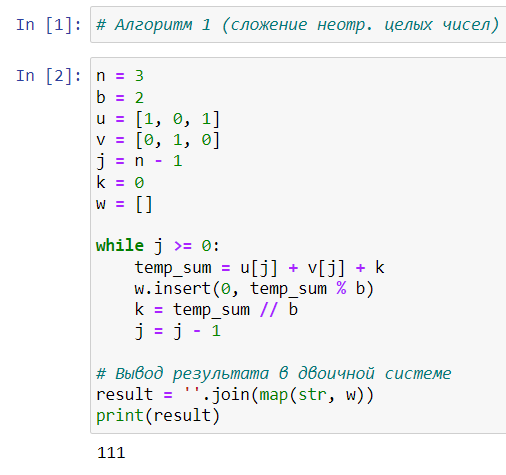
\includegraphics[width=0.8\textwidth,height=\textheight]{./tex2pdf.-e48f57e5a48111ba/image/1.png}
\caption{Алгоритм Евклида}\label{fig:001}
\end{figure}

\section{Бинарный алгоритм
Евклида}\label{ux431ux438ux43dux430ux440ux43dux44bux439-ux430ux43bux433ux43eux440ux438ux442ux43c-ux435ux432ux43aux43bux438ux434ux430}

\subsection{Задача}\label{ux437ux430ux434ux430ux447ux430-1}

Реализовать бинарный алгоритм Евклида

\subsubsection{Решение}\label{ux440ux435ux448ux435ux43dux438ux435-1}

Реализуем бинарный алгоритм Евклида (рис. \ref{fig:002})

\begin{figure}
\centering
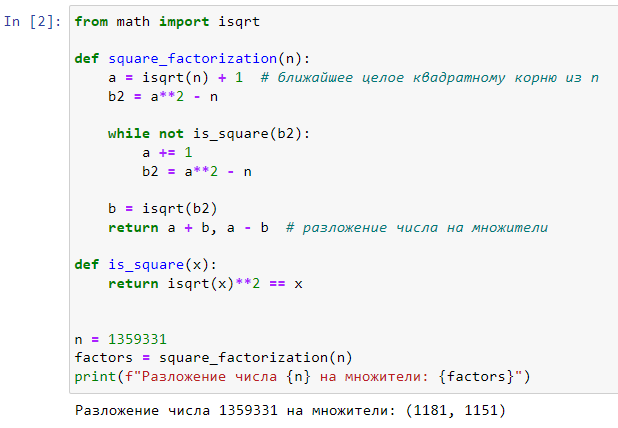
\includegraphics[width=0.8\textwidth,height=\textheight]{./tex2pdf.-e48f57e5a48111ba/image/2.png}
\caption{Бинарный алгоритм Евклида}\label{fig:002}
\end{figure}

\section{Расширенный алгоритм
Евклида}\label{ux440ux430ux441ux448ux438ux440ux435ux43dux43dux44bux439-ux430ux43bux433ux43eux440ux438ux442ux43c-ux435ux432ux43aux43bux438ux434ux430}

\subsection{Задача}\label{ux437ux430ux434ux430ux447ux430-2}

Реализуем расширенный алгоритм Евклида (рис. \ref{fig:003})

\begin{figure}
\centering
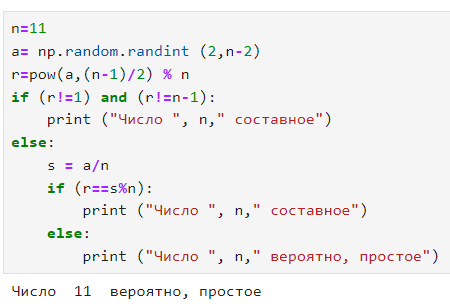
\includegraphics[width=0.8\textwidth,height=\textheight]{./tex2pdf.-e48f57e5a48111ba/image/3.png}
\caption{Расширенный алгоритм Евклида}\label{fig:003}
\end{figure}

\section{Расширенный бинарный алгоритм
Евклида}\label{ux440ux430ux441ux448ux438ux440ux435ux43dux43dux44bux439-ux431ux438ux43dux430ux440ux43dux44bux439-ux430ux43bux433ux43eux440ux438ux442ux43c-ux435ux432ux43aux43bux438ux434ux430}

\subsection{Задача}\label{ux437ux430ux434ux430ux447ux430-3}

Реализуем расширенный бинарный алгоритм Евклида (рис. \ref{fig:004})

\begin{figure}
\centering
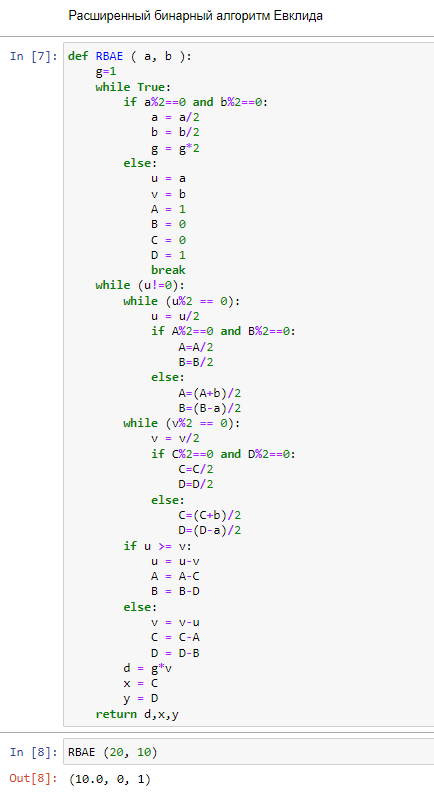
\includegraphics[width=0.8\textwidth,height=\textheight]{./tex2pdf.-e48f57e5a48111ba/image/4.png}
\caption{Расширенный бинарный алгоритм Евклида}\label{fig:004}
\end{figure}

\chapter{Выводы}\label{ux432ux44bux432ux43eux434ux44b}

В ходе данной лабораторной работы я рассмотрел и реализовал следующие
алгоритмы:

\begin{itemize}
\item
  Алгоритм Евклида;
\item
  Бинарный алгоритм Евклида;
\item
  Расширенный алгоритм Евклида;
\item
  Расширенный бинарный алгоритм Евклида.
\end{itemize}

\chapter{Библиография}\label{ux431ux438ux431ux43bux438ux43eux433ux440ux430ux444ux438ux44f}

\begin{enumerate}
\def\labelenumi{\arabic{enumi}.}
\item
  Python documentation. {[}Электронный ресурс{]}. М. URL:
  \href{https://docs.python.org/3/index.html}{Python documentation}
  (Дата обращения: 28.09.2023).
\item
  Лабораторная работа №4. Вычисление НОД. - 4 с. {[}Электронный
  ресурс{]}. М. URL:
  \href{https://esystem.rudn.ru/pluginfile.php/2089804/mod_folder/content/0/lab04.pdf}{Лабораторная
  работа №4. Вычисление НОД.} (Дата обращения: 19.10.2023).
\end{enumerate}

\printbibliography

\end{document}
